\subsubsection{General program description}
In this example we solve an optimization problem where 
the equations come from fluid-structure interaction (FSI). The idea
is to extend the steady FSI benchmark problem (FSI 1, proposed by Hron/Turek) 
to an optimization 
problem where the drag is minimized over the cylinder and the beam. 
The setting is similar to Opt Example 3. In fact, the only 
novel things are to attach an elastic beam at the cylinder and to 
extend the equation to fluid-structure interaction (instead of 
pure fluid as in Example 3).

\begin{figure}[h]
\centering
    {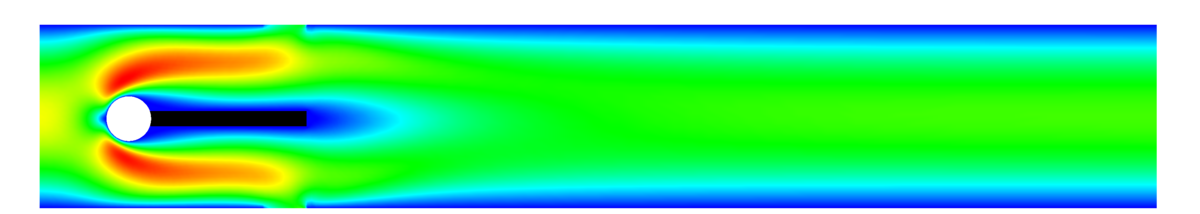
\includegraphics[width=7cm]{Documentation/visit_fsi_1_opt_control_p3_0002_bearbeitet_Aug_15.png}}
    {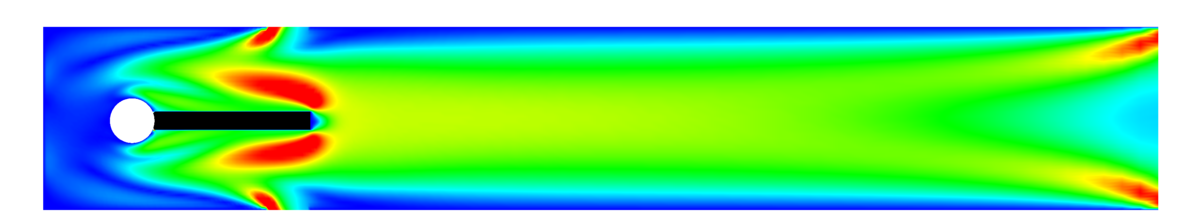
\includegraphics[width=7cm]{Documentation/visit_fsi_1_opt_control_p3_0005_bearbeitet_Aug_15.png}}
  \caption{Configuration of the FSI cylinder-beam-drag minimization problem. 
By sucking out the fluid, 
the force on the cylinder is reduced. At left, the $x$-velocity field 
is shown. In right figure, we the corresponding adjoint solution is shown.}
\end{figure}

The state equation system reads:
\begin{Problem}[Stationary Fluid-Structure Interaction with STVK material]
Let $q$ denote the control variable. Find $U:= \{\hat v,\hat p,\hat u\}$ such that
  \begin{equation*}
    \begin{aligned}
      (\hat J \rho_f \hat F^{-1}\hat  v\cdot\hat\nabla \hat v,
      \hat\phi^v)_{\hat\Omega_f}
      + (\hat J\hat\sigma_f\hat F^{-T},\hat \nabla\hat\phi^v)_{\hat\Omega_f}\\
      + (\hat J\hat\sigma_s\hat F^{-T},\hat \nabla\hat\phi^v)_{\hat\Omega_s}
      + \langle q,\hat\phi^v\cdot \hat n\rangle_{\Gamma_Q}
      &= 0&&\forall\hat\phi^v\in \hat V,\\
      %%%%%%%%%%%% 
      (\hat v,\hat\phi^u)_{\hat\Omega_s}
      + (\alpha_u \hat \nabla \hat u,\hat \nabla\hat\phi^u)_{\hat\Omega_f}
      &=0&&\forall\hat\phi^u\in \hat V,\\
    %%%%%%%%%%%%%%%%%%%%%%%%%%%%%%
      (\widehat{\text{div}}\,(\hat J\hat F^{-1}\hat
      v_f),\hat\phi^p)_{\hat\Omega_f} 
      + (\hat p,\hat \phi^p)_{\hat\Omega_s}
      &=0&&\forall\hat \phi^p\in \hat L,
    \end{aligned}
  \end{equation*}  
\end{Problem}

The target functional is considered as 
\[
k(U) = \int_{\hat\Gamma_O \cup \hat\Gamma_i} \hat n\cdot \hat J\hat\sigma(v,p)\hat
F^{-T} \cdot \hat d \, ds,
\]
where $\Gamma_O$ denotes the cylinder boundary and $\Gamma_i$ the 
interface between fluid and solid, and $\hat d$ is a vector in the
direction
of the mean flow. Moreover, $\hat J$ and $\hat F$ denote the deformation 
gradient and its determinant as well known in fluid-structure interaction.
For theoretical and numerical reasons, this functional 
needs to be regularized, including the control variable $q$, such that
\[
K(q,U) = k(U) + \frac{\alpha}{2}||q - q_0||^2,
\] 
where $\alpha$ is the Tikhonov parameter and $q_0$ some 
reference control. 

The rest of the program is similar to the previous optimization problems where
we formulate the state equation in a weak form $a(q,U)(\phi)$ such that the 
final problem reads
\[
K(q,U) \rightarrow \text{min} \quad \text{s.t.} \quad a(q,U)(\phi) = 0.
\]

\subsubsection{Program description}
This example is similar to Example \ref{OPT_Stat_Param_Nonlin_Fluid} (both 
based on Example \ref{OPT_Stat_Param_Lin_Ellipt}), except that we 
have again much more complicated (nonlinear) equations. A modification 
of this example and several numerical tests are presented 
in \cite{RiWi13_fsi_opt}.






